\documentclass[tikz,border=10pt]{standalone}
\usepackage{xcolor}

\begin{document}
\sffamily

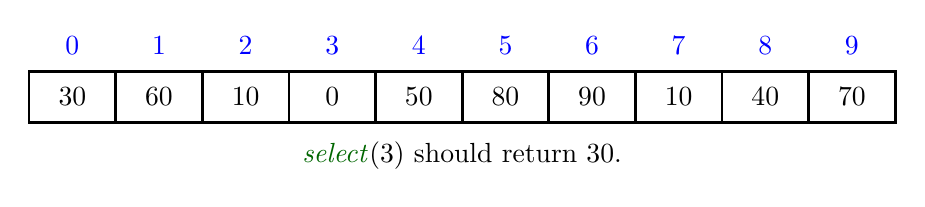
\begin{tikzpicture}[
  cell/.style={draw, line width=1pt, minimum width=1.1cm,
               minimum height=0.65cm, inner sep=0pt}
]
  % Array cells and blue indices above them
  \foreach \v [count=\i from 0] in {30,60,10,0,50,80,90,10,40,70} {
    \node[cell] at (\i*1.1, 0) {\v};
    \node[blue] at (\i*1.1, 0.65) {\i};
  }

  % Caption centered under the array
  \node at (4.95,-0.75)
    {{\color{green!40!black}\textit{select}}(3) should return 30.};
\end{tikzpicture}

\end{document}
